\documentclass{article}

\usepackage{graphicx}
\usepackage{float}
\usepackage{amsmath}

%The following package imports and styling was obtained from: https://tex.stackexchange.com/questions/348651/c-code-to-add-in-the-document
\usepackage{xcolor}
\usepackage{listings}

\definecolor{mGreen}{rgb}{0,0.6,0}
\definecolor{mGray}{rgb}{0.5,0.5,0.5}
\definecolor{mPurple}{rgb}{0.58,0,0.82}
\definecolor{backgroundColour}{rgb}{0.95,0.95,0.92}

\usepackage[colorlinks]{hyperref}
\hypersetup{citecolor=DeepPink4}
\hypersetup{linkcolor=DarkRed}
\hypersetup{urlcolor=blue}
\usepackage{cleveref}

\lstdefinestyle{CStyle}{
    backgroundcolor=\color{backgroundColour},   
    commentstyle=\color{mGreen},
    keywordstyle=\color{magenta},
    numberstyle=\tiny\color{mGray},
    stringstyle=\color{mPurple},
    basicstyle=\footnotesize,
    breakatwhitespace=false,         
    breaklines=true,                 
    captionpos=b,                    
    keepspaces=true,                 
    numbers=left,                    
    numbersep=5pt,                  
    showspaces=false,                
    showstringspaces=false,
    showtabs=false,                  
    tabsize=2,
    language=C
}

\begin{document}
\title{Sfwr Eng 4F03: Final Project}

\author{Kelvin Lin\hspace{10mm}MacID:linkk4\hspace{10mm}Student Number: *********\\Prabhbir Pooni\hspace{10mm}MacID: poonip\hspace{10mm}Student Number: *********\\Yanting Zhang\hspace{10mm}MacID: zhang169\hspace{10mm}Student Number: *********}

\maketitle

\section{Question 1}
Using \texttt{MPIHost}, timing, speed-up, and efficiency plots were generated for 1, 2, 4, 8, 16, and 32 processors. The program was tested with 2000, 4000, 8000, 16000, and 32000 particles. 9 major steps were used with 1 substep in between. The image produced was 2550 pixels in width by 1960 pixels in height.

For each section, two graphs will be presented. The first graph shows metrics for a pure MPI implementation, while the second graph shows metrics for an MPI implementation optimized with OpenMP.

\subsection{Timing Plot}
The following graphs are timing plots for the different image sizes, different number of particles, and different number of processors. Each line represents a different number of particles. The x-axis represents the number of processors while the y-axis represents the time it took to run the program.

\subsubsection{Pure MPI}
\begin{figure}[H]
	\begin{center}
		\hspace*{-0.5cm}                                                           
  		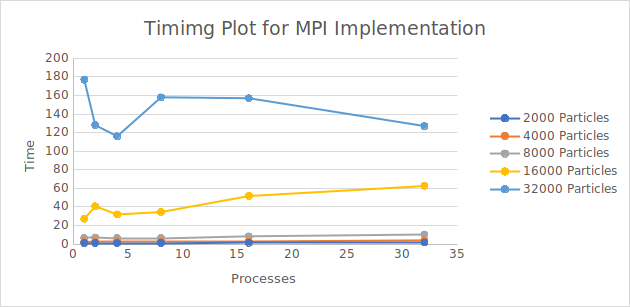
\includegraphics[scale=0.83]{Report_Assets/timingmpi.png}
  	\end{center}
  	\caption{The timing plot with varying the number of processors and particles in MPI}
\end{figure}

\subsubsection{MPI Optimized with OpenMP}
\begin{figure}[H]
	\begin{center}
		\hspace*{-0.5cm}                                                           
  		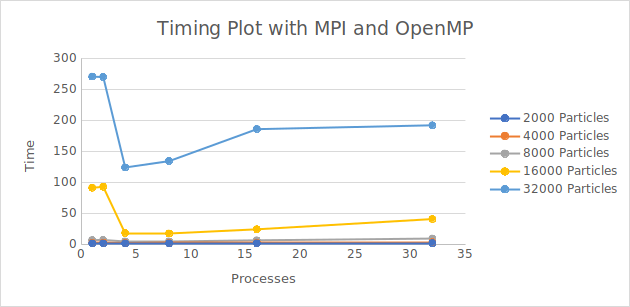
\includegraphics[scale=0.83]{Report_Assets/timingomp.png}
  	\end{center}
  	\caption{The timing plot with varying the number of processors and particles in MPI with OpenMP}
\end{figure}

\subsection{Speedup Plot}
The following graphs are speedup plots for the different image sizes, different number of particles, and different number of processors.

Each line represents a different number of particles. The x-axis represents the number of processors used, while the y-axis represents the speedup observed.

\subsubsection{Pure MPI}
\begin{figure}[H]
	\begin{center}
		\hspace*{-0.5cm}                                                           
  		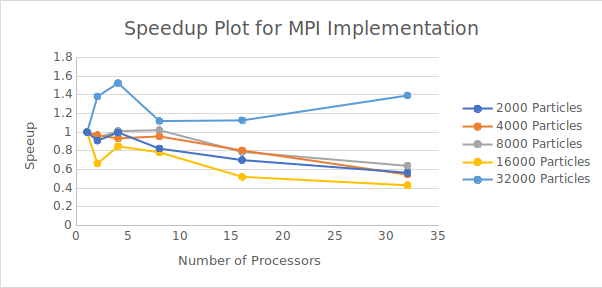
\includegraphics[scale=0.71]{Report_Assets/speedupmpi.png}
  	\end{center}
  	\caption{The speedup plot with varying the number of processors and particles in MPI}
\end{figure}

\subsubsection{MPI Optimized with OpenMP}
\begin{figure}[H]
	\begin{center}
		\hspace*{-0.5cm}                                                           
  		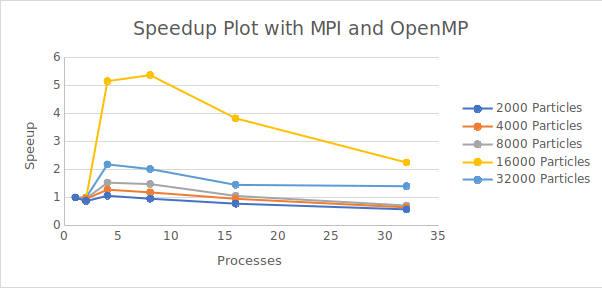
\includegraphics[scale=0.71]{Report_Assets/speedupomp.png}
  	\end{center}
  	\caption{The speedup plot with varying the number of processors and particles in MPI with OpenMP}
\end{figure}

\newpage
\subsection{Efficiency Plot}
The following graphs are efficiency plots for the different image sizes, different number of particles, and different number of processors.

Each line represents a different number of particles. The x-axis represent the different number of processors used, while the y-axis represents the efficiency.

\subsubsection{Pure MPI}
\begin{figure}[H]
	\begin{center}
		\hspace*{-0.5cm}                                                           
  		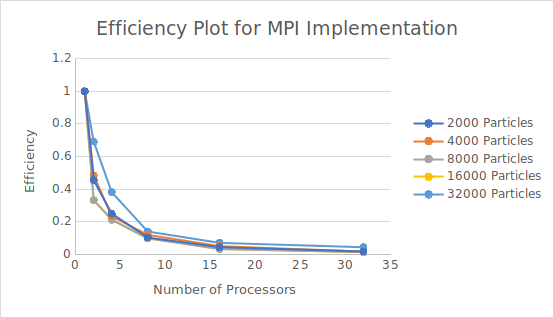
\includegraphics[scale=0.65]{Report_Assets/efficiencympi.png}
  	\end{center}
  	\caption{The efficiency plot with varying the number of processors and particles in MPI}
\end{figure}

\subsubsection{MPI Optimized with OpenMP}
\begin{figure}[H]
	\begin{center}
		\hspace*{-0.5cm}                                                           
  		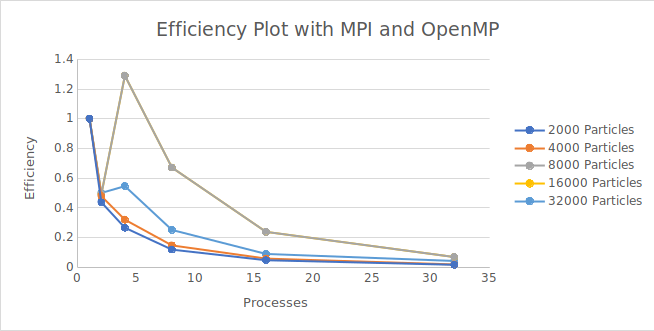
\includegraphics[scale=0.6]{Report_Assets/efficiencyomp.png}
  	\end{center}
  	\caption{The efficiency plot with varying the number of processors and particles in MPI with OpenMP}
\end{figure}

\section{Question 2}
\subsection{Strong Scalability}
A strongly scalable algorithm is an algorithm where given a fixed problem size, as the number of processors increase, the efficiency stays about the same.

If an algorithm is strongly scalable, then an approximately straight horizontal line should be observed in Figure 5. Figure 5 shows whether an alogirithm is strongly scalable because each line shows the efficiency of the processors for a fixed problem size as the number of processors used increases.

From Figure 5, it is clear that the efficiency decreases in an exponential fashion for all input sizes. Accordingly, the algorithm is not strongly scalable.

\end{document}
